% This file is a valid PHP file and also a valid LaTeX file
% When processed with LaTeX, it will generate a blank template
% Loading with PHP will fill it with details

\documentclass[12pt,a4paper]{article}
% Required for proper escaping
\usepackage[left=2.5cm,right=2.5cm,top=2.5cm,bottom=2.5cm]{geometry}
%\usepackage{ctex}
%\XeTeXlinebreaklocale "zh"
%\XeTeXlinebreakskip = 0pt plus 1pt
\usepackage{CJK}
\usepackage{graphicx}
\graphicspath{{/home/www/html/iscs/latex/hw6}}
% Make placeholders visible
\newcommand{\placeholder}[1]{\textbf{$<$ #1 $>$}}

% Defaults for each variable
\newcommand{\idnumber}{\placeholder{Student ID}}
\newcommand{\moodleid}{\placeholder{ID}}


% Fill in
% <?php echo "\n" . "\\renewcommand{\\idnumber}{" . CLatexTemplate::escape($data['idnumber']) . "}\n"; ?>
% <?php echo "\n" . "\\renewcommand{\\moodleid}{" . CLatexTemplate::escape($data['moodleid']) . "}\n"; ?>

% LaTeX code for the invoice
\usepackage{tabularx}
\setlength{\parindent}{0pt}
\pagestyle{empty}
\usepackage{amsmath}
\usepackage{amssymb}


\begin{document}
\begin{CJK}{UTF8}{bsmi}
\begin{flushleft}Introduction to Scientific Computing Software HW6
\\Student ID : \idnumber{}\end{flushleft}

請利用上週程式碼來完成作業。以下的 $t$ 皆是 $t=1:44100$
\begin{enumerate}
\item 請造出一個陣列長度為 44100 的方波
\begin{itemize} 


\item $f_1(t)=\left\{\begin{array}{ll}0.5&,0 \le t < 50 \\ -0.5 &,50 \le t < 100\end{array}\right.$
\item $f_1(t)=f_1(t+100)$
\end{itemize}
\item 請造出一個陣列長度為 44100 的 $\sin$ 波
\begin{itemize}

\item $f_2(t)=2\sin(2\pi \cdot t/100)$
\end{itemize}

\item 利用邏輯陣列來造出以下新的波
\begin{itemize}

\item $f_3(t)=\left\{\begin{array}{ll}0.5&, f_2>10^{-10}\ \mbox{and}\ f_2>f_1 \\ -0.5 &,f_2<-10^{-10}\ \mbox{and}\ f_2<f_1 \\f_2(t) & ,\mbox{otherwise} \end{array}\right.$
\item 示意圖 \\ 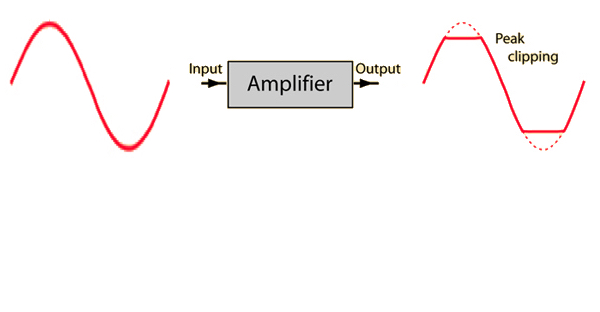
\includegraphics[width=12cm]{amp2-1}
\end{itemize}
\item 繳交格式
\begin{itemize}
\item  畫出 $f_3$ 與 $f_2$ 的疊圖
\item  範圍 $12345\le t \le 12845, -3\le y \le 3$
\item  $f_3$圖使用 '.' 樣式
\item ``學號.m檔"、``結果截圖"請一起放進資料夾,使用zip壓縮
\item  檔名:學號.zip
\item  plot函數的title: 學號  姓名
\end{itemize}
\end{enumerate}
\end{CJK}
\end{document}
